\begin{frame}{飛行距離は季節で 3.5 倍変わる}{結果：北海道の落下位置}
  \begin{columns}[T]
    \begin{column}{0.34\textwidth}
      \begin{center}
      \begin{tikzpicture}[x=1mm,y=1mm,>={Latex[length=2mm,width=1.6mm]}]
        \draw[wcMuted,line width=0.6pt] (0,0) -- (44,0);
        \draw[wcMuted,line width=0.5pt,dotted] (0,5) -- (44,5);
        \draw[wcMuted,line width=0.5pt,dotted] (0,10) -- (44,10);
        \node[font=\fontsize{8}{9}\selectfont,text=wcMuted,anchor=east] at (43.5,7.5) {層 $k$};
        \draw[wcBlue,line width=1.6pt,->] (2,0) -- (14,15);
        \node[font=\fontsize{8.5}{9.5}\selectfont,text=wcBlue,anchor=east,align=right] at (7.5,8.5) {上昇\\5 m/s};
        \fill[wcOrange] (14,15) circle (1.2);
        \node[font=\mediumfont\fontsize{8.5}{10}\selectfont,text=wcOrange,anchor=south] at (14,16.2) {破裂 30 km};
        \draw[wcBlue,line width=1.6pt,dashed,->] (14,15) -- (34,0);
        \node[font=\fontsize{8.5}{9.5}\selectfont,text=wcBlue,anchor=west,align=left] at (25,8.5) {降下\\6 m/s};
        \draw[wcSecondary,line width=0.7pt,<->] (2,-2.5) -- (34,-2.5);
        \node[font=\fontsize{8.5}{9.5}\selectfont,text=wcSecondary,anchor=north] at (18,-3) {$\Delta x$、約 137 分};
      \end{tikzpicture}
      \end{center}
      \vskip 0.5mm
      \sub{$\Delta x = \sum_k u_k T_k$\\$T_k$ は層 $k$ の滞在時間}
    \end{column}
    \begin{column}{0.64\textwidth}
      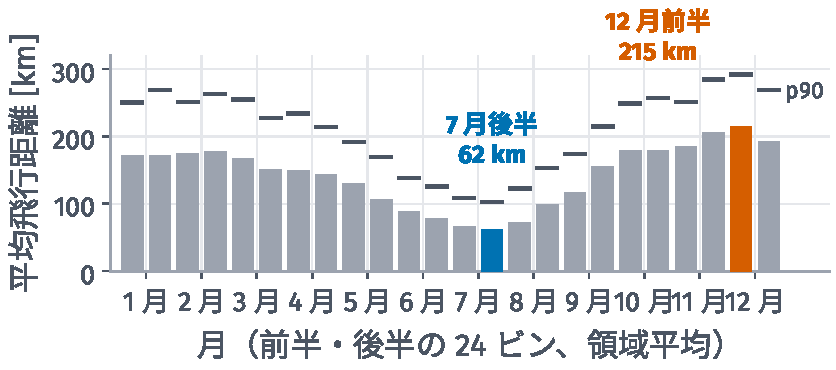
\includegraphics[width=\linewidth,height=108pt,keepaspectratio]{S_drift_by_bin.pdf}
      \vskip 0.5mm
      \sub{領域平均、進行方位は東北東でほぼ一定。\\11--12 月は平均 200 km 超、p90 は 300 km。}
    \end{column}
  \end{columns}
  \srcline{飛行モデルは既存シミュレータと同一。$T_k$ は風によらない}
\end{frame}
